\section{Introduction}



% ----------1.1----------
\subsection{Some Representative Time Series}
We begin with some examples of the sort of time series that arise in practice.

\textit{Economic and financial time series}

Many time series are routinely recorded in economics and finance: Share prices on succesive days, export totals in successive months, average incomes in successive months, company profits in successive years, and so on.

The classic Beveridge wheat price index series consists of the average wheat price in nearly 50 places in various countries measured in successive years from 1500 to 1869. We can plot the series via 
\begin{minted}{R}
> library(tseries) # load the library
> data(bev) # load the dataset
> plot(bev, xlab="Year", ylab="Wheat price index", xaxt="n")
> x.pos = c(1500, 1560, 1620, 1680, 1740, 1800, 1860) # define x-axis labels
> axis(1, x.pos, x.pos)
\end{minted}
\cref{fig:1.1} shows this series and some apparent cyclic behavior can be seen.

\begin{figure}[h]
	\centering
	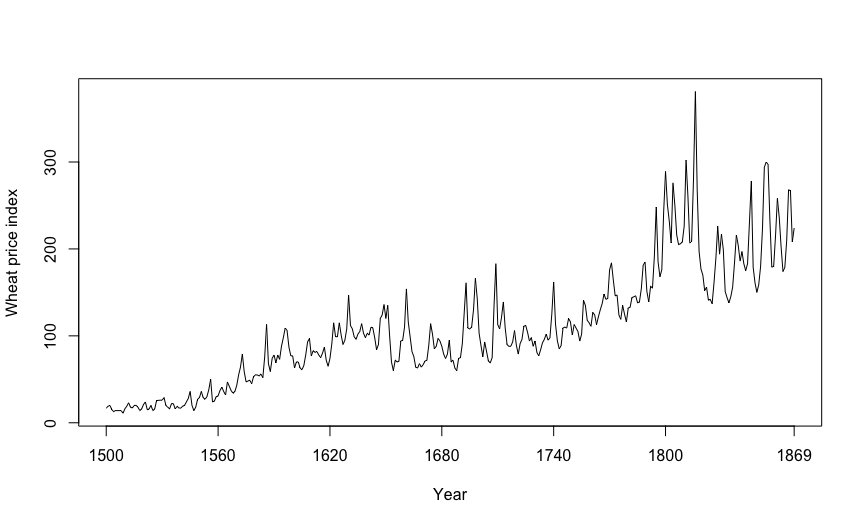
\includegraphics[width=0.8\textwidth]{Chapter 1/fig1-1.png}
	\caption{The Beverage wheat price annual index series from 1500 to 1869.}
	\label{fig:1.1}
\end{figure}

There is also an example of financial time series: \cref{fig:1.2} below hsows the daily returns (or percentage change) of the adjusted closing prices of the Standard \& Poor's 500 (S\&P) Index from January 4th, 1995 to December 30th, 2016.

\begin{figure}[ht]
	\centering
	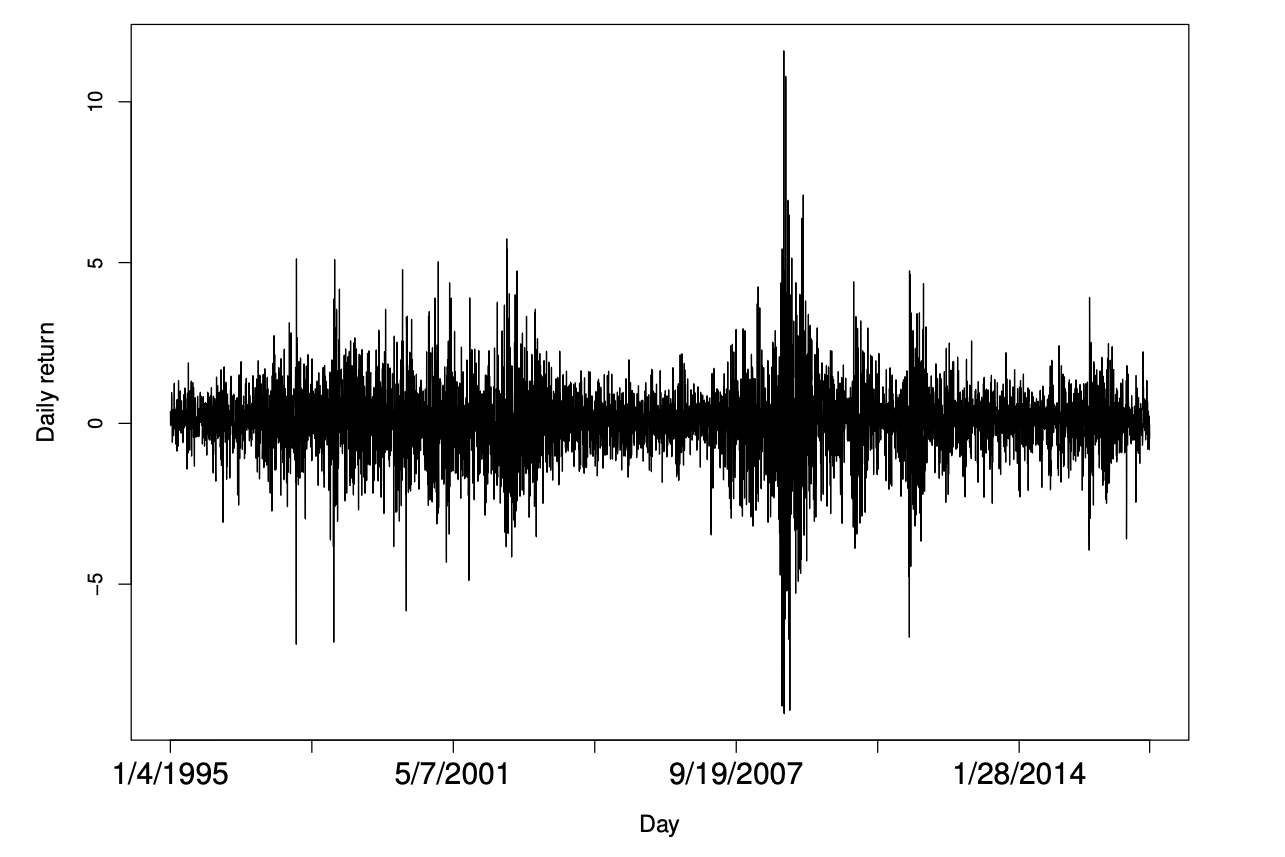
\includegraphics[width=0.8\textwidth]{Chapter 1/fig1-2.png}
	\caption{Daily returns of the adjusted closing proces of the S\&P index from January 4th, 1995 to December 40th, 2016.}
	\label{fig:1.2}
\end{figure}

To reproduce \cref{fig:1.2} in R, suppose we have the data as \lstinline{sp500\_ret\_1995-2016.csv} in the directory \lstinline{mydata}. Then we can load the data via the following piece of code:

\begin{minted}{R}
> sp500<-read.csv("mydata/sp500\_ret\_1995-2016.csv")
> n<-nrow(sp500)
> x.pos<-c(seq(1,n,800),n)
> plot(sp500\$Return, type="l", xlab="Day", ylab="Daily return", xaxt="n")
> axis(1, x.pos, sp500\$Date[x.pos])
\end{minted}

\textit{Physical time series}
Many types of times series occur in the physical sciences, particularly in meteorology, marine sciences, and geophysics. Examples are rainfall on succesive days, and air temperature measured in successive hours, days, or months. \cref{fig:1.3} shows the average air temperature in Anchorage, Alaska in the US in successive months over a 16 year time period. The series can be downloaded from the U.S. National Centers for Environmental Information. Seasonal fluctuations can be clearly seen in the series.

\begin{figure}[h]
	\centering
	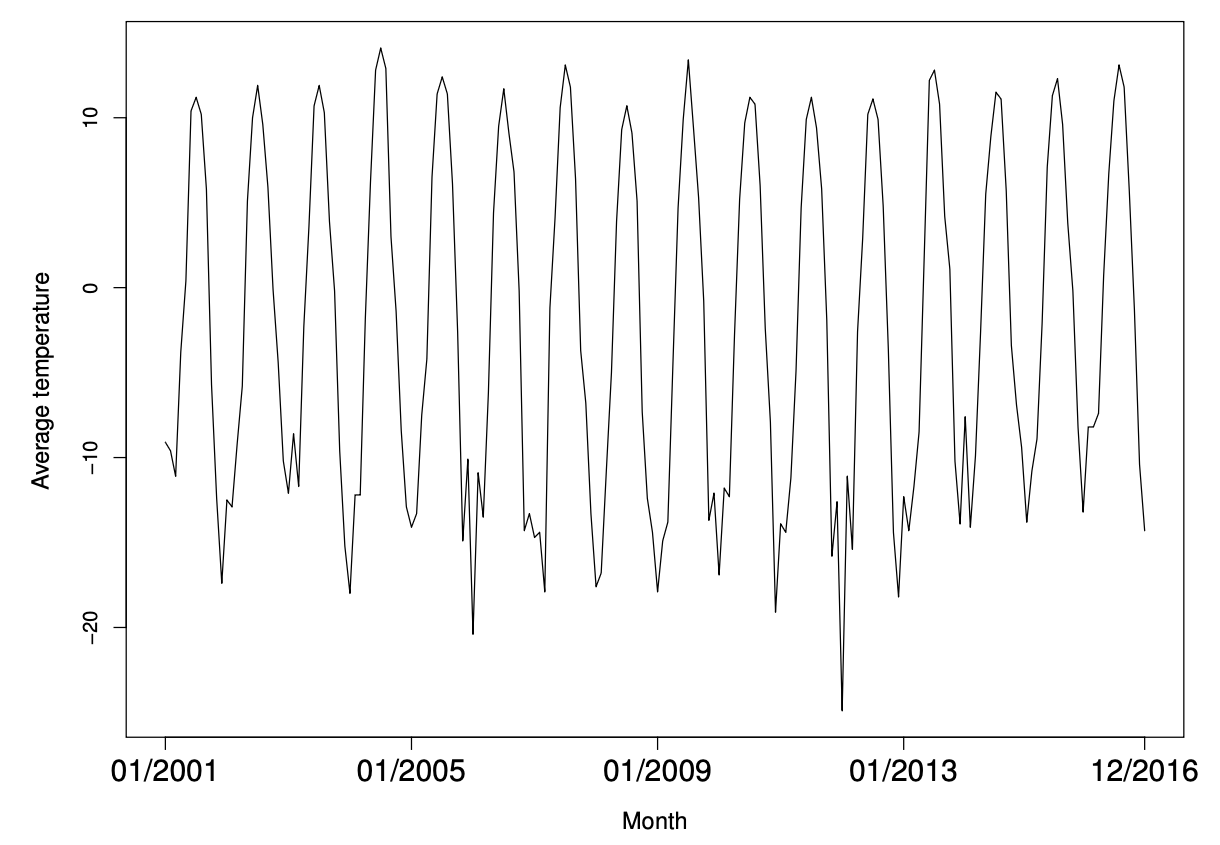
\includegraphics[width=0.65\textwidth]{Chapter 1/fig1-3.png}
	\caption{Monthly average air temperature (degrees Celcius) in Anchorage, Alaska, in successive months from 2001 to 2016.}
	\label{fig:1.3}
\end{figure}

Some mechanical recorders take measurements continuously and produce a continuous trace rather than observations at discrete intervals of time. However, for more detailed analysis, it is customary to convert the continuous trace to a series in discrete time by sampling the trace at appropriate intervals of time. The resulting analysis is more straightforward and can be handled by standard time series software.

\textit{Marketing time series}

The analysis of time series arising in marketing is an important problem in commerce. Observed variables could include sales figures in successive weeks or months, monetary receipts, advertising costs and so on. As an example, 
\cref{fig:1.4} shows the domestic sales of Australian fortified wine by winemakers in successive quarters over a 30-year period, which are available at the Australian Bureau of Statistics.

\begin{figure}[ht]
	\centering
	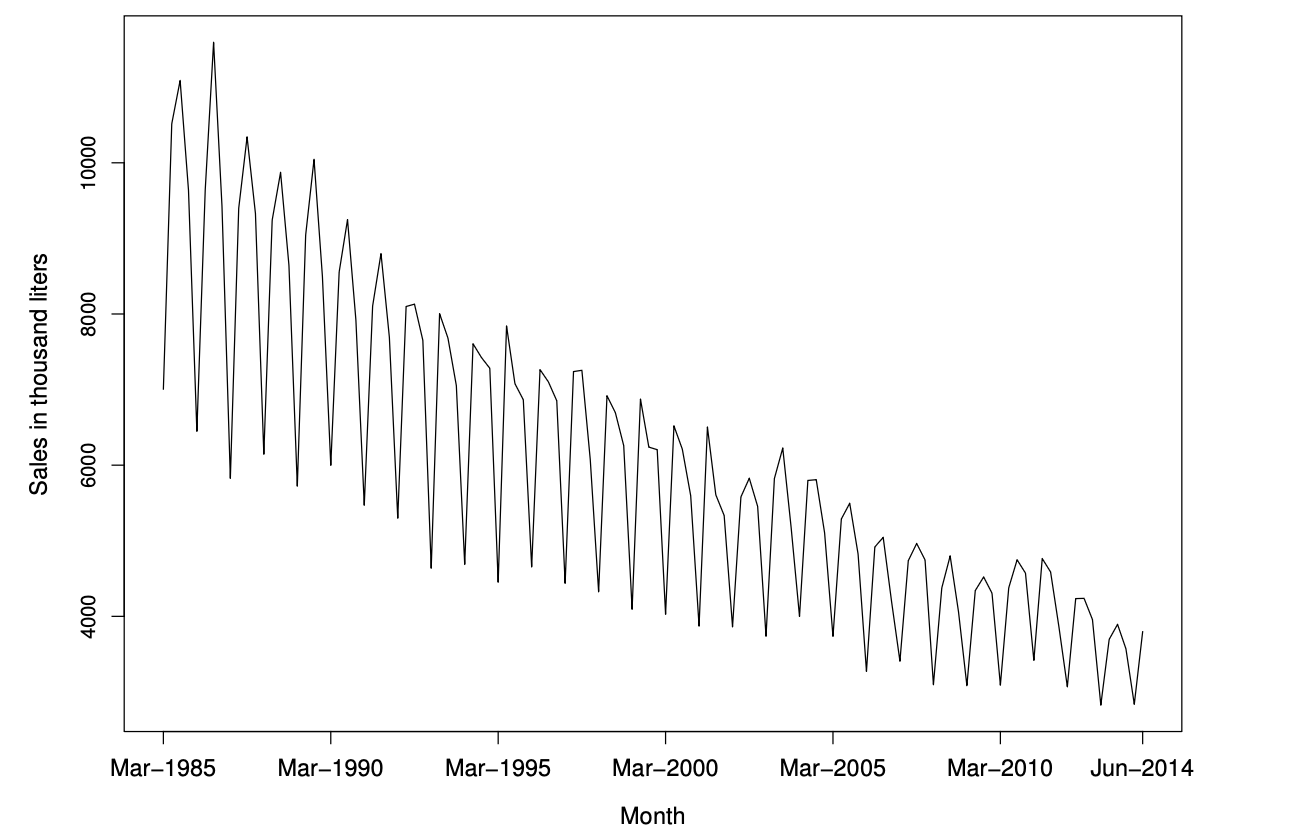
\includegraphics[width=0.8\textwidth]{Chapter 1/fig1-4.png}
	\caption{Domestic sales (unit: thousand liters) of Australian fortified wine by winemakers in successive quarters from March 1985 to June 2014.}
	\label{fig:1.4}
\end{figure}

Note the trend and seasonal variation above.

\textit{Demographic time series}

Various time series occur in the study of population change. Examples include the total population of Canada measured annually, and monthly birth totals in England. \cref{fig:1.5} shows the total population and crude birth rate (per 1000 people) for the UNited States from 1965 to 2015. The data are available at the US Federal Reserve Bank of St. Louis.

\begin{figure}[h]
	\centering
	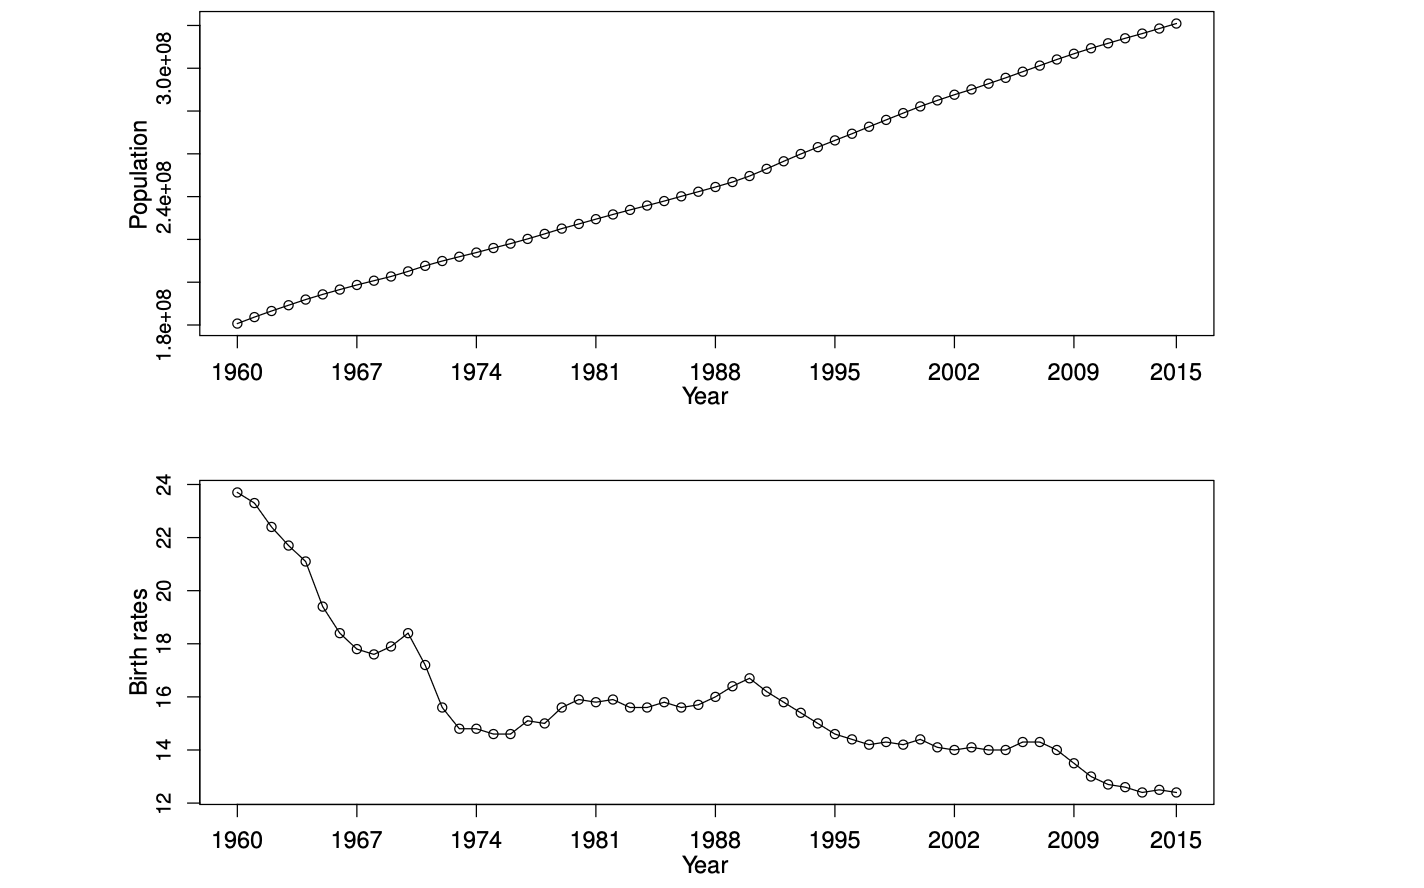
\includegraphics[width=0.8\textwidth]{Chapter 1/fig1-5.png}
	\caption{Total population and birth rate (per 1000 people) for the United States from 1965 to 2015.}
	\label{fig:1.5}
\end{figure}

We can reproduce \cref{fig:1.5} using the following piece of code:
\begin{minted}{R}
> pop<-read.csv("mydata/US\_pop\_birthrate.csv", header=T)
> x.pos<-c(seq(1, 56, 7), 56)
> x.label<-c(seq(1960, 2009, by=7), 2015)

> par(mfrow=c(2,1), mar=c(3,4,3,4))
> plot(pop[,2], type="l", xlab="", ylab="", xaxt="n")
> points(pop[,2])
> axis(1, x.pos, x.label, cex.axis=1.2)
> title(xlab="Year", ylab="Population", line=2, cex.lab=1.2)

> plot(pop[,3], type="l", xlab="", ylab="", xaxt="n")
> points(pop[,3])
> axis(1, x.pos, x.label, cex.axis=1.2)
> title(xlab="Year", ylab="Birth rates", line=2, cex.lab=1.2)
\end{minted}

\textit{Process control data}

In process control, a problem is to detect changes in the performance of a manufacturing process by measuring a variable, which shows the quality of the process. These measurements can be plotted against time, as shown in \cref{fig:1.6} below.

\begin{figure}[h]
	\centering
	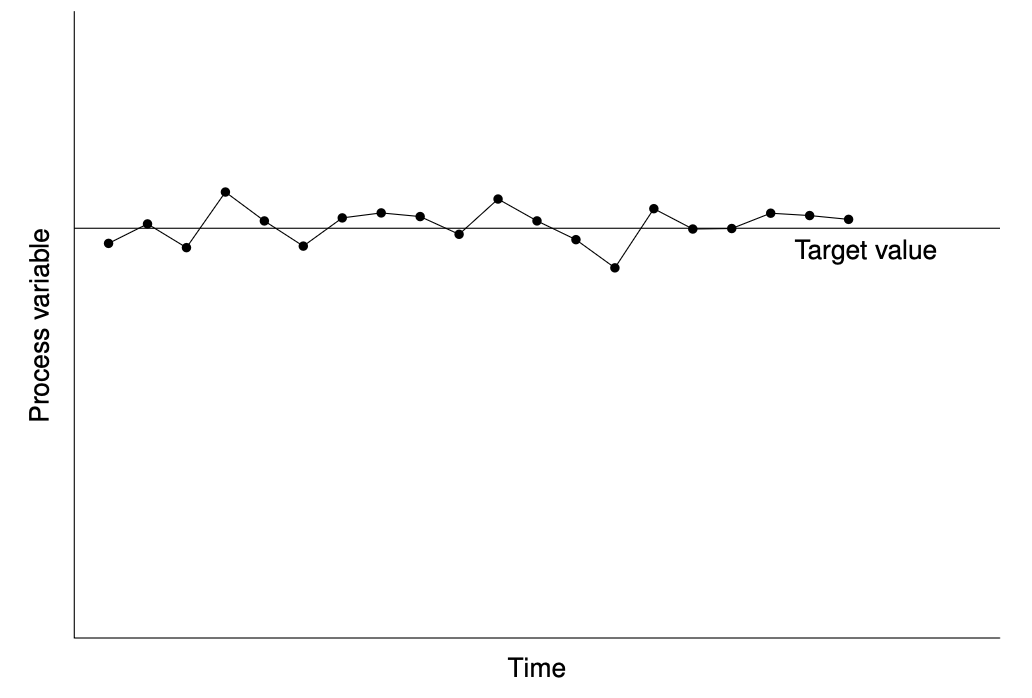
\includegraphics[width=0.8\textwidth]{Chapter 1/fig1-6.png}
	\caption{A process control chart.}
	\label{fig:1.6}
\end{figure}

Special techniques have been developed for this type of time series problems, namely statistical quality control (Montgomery, 1996).

\textit{Binary processes}
A special type of time series arisis when observations can only take one of only two values, usually denoted by 0 and 1 (see \cref{fig:1.7}). For example, in computer science, the position of a switch could be recorded as 1 or 0 respectively.


Time series of this type occur in many situations, including the study of communication theory. A problem here is to predict when the process will take a different value.

\textit{Point processes}
We can consider a series of events occuring `randomly' through time, such as the dates of major railway disasters. A series of events of this type is usualled called a point process. As an example, \cref{fig:1.8} shows the intraday transaction data of the International Business Machines (IBM) Corporation from 9:35:00 to 9:38:00 on January 4th, 2010. When a trade event occurs, the corresponding trading price and trading volume are observed.

Methods of analyzing point process data are generally very different from those used for analyzing standard time series data. The text by Cox and Isham (1980) is recommended.

\newpage
\begin{figure}[ht]
	\centering
	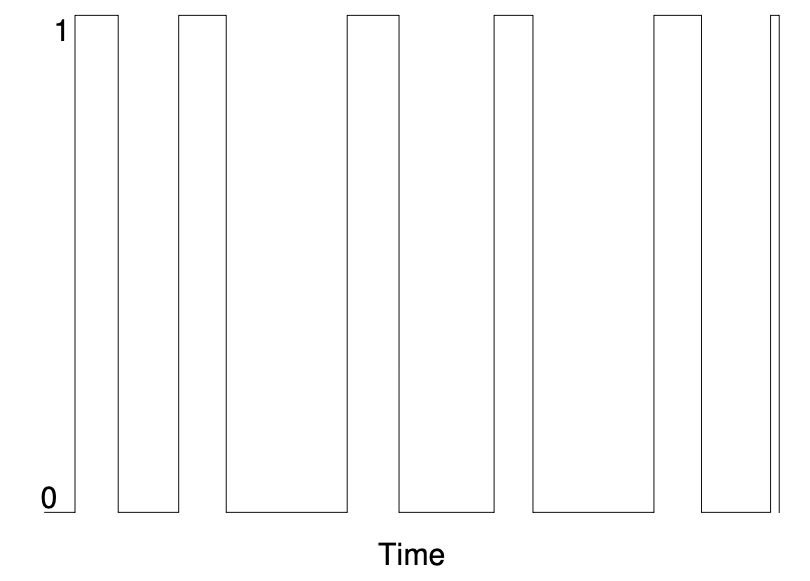
\includegraphics[width=0.7\textwidth]{Chapter 1/fig1-7.png}
	\caption{A realization of a binary process.}
	\label{fig:1.7}
\end{figure}

\begin{figure}[h]
	\centering
	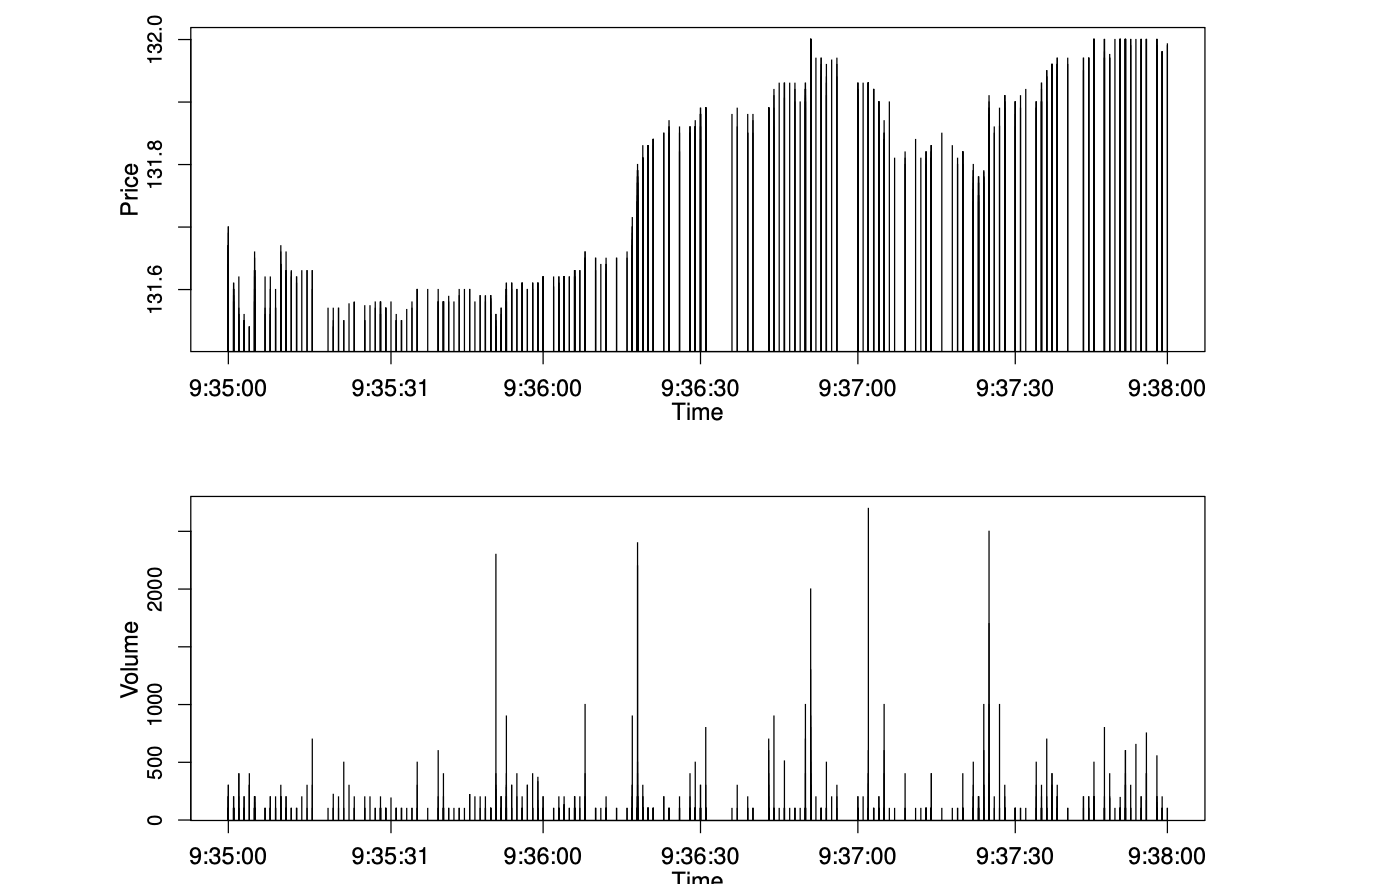
\includegraphics[width=0.8\textwidth]{Chapter 1/fig1-8.png}
	\caption{Transaction prices and volumes of the IBM stocks from 9:35:00 to 9:38:00 on January 4th, 2010.}
	\label{fig:1.8}
\end{figure}

\newpage
To reproduce \cref{fig:1.8}, we can use the following piece of code:
\begin{minted}{R}
> ibm<-read.table("mydata/taq\_trade\_ibm\_100104.txt",
header=T, sep="\t")
> ibm.new<-ibm[,c(1,2,7)]
> ibm[,2]<-as.numeric(as.character(ibm[,2]))

> ### take 9:35:00-9:37:59am trading record
> data<-ibm.new[1458:2371,]
> newtime<-rep(0, nrow(data))
> for (i in 1:nrow(data)){
  min<-as.numeric(substr(as.character(data\$TIME[i]),3,4))
  sec<-as.numeric(substr(as.character(data\$TIME[i]),6,7))
  newtime[i]<- (min-30)*60+sec
}

> x.label<-c("9:35:00", "9:35:31", "9:36:00", "9:36:30",
"9:37:00", "9:37:30", "9:38:00")
> x.pos<-c(1, 139, 249, 485, 619, 776, 914)
> par(mfrow=c(2,1), mar=c(2,4,2,4))

> plot(newtime, data[,2],xlab="",ylab="",xaxt="n",type="h")
> axis(1, newtime[x.pos], x.label, cex.axis=1.2)
> title(xlab="Time", ylab="Price", line=2, cex.lab=1.2)
> plot(newtime, data[,3],xlab="",ylab="",xaxt="n",type="h")
> axis(1, newtime[x.pos], x.label, cex.axis=1.2)
> title(xlab="Time", ylab="Volume", line=2, cex.lab=1.2)
\end{minted}



% ----------1.2----------
\subsection{Terminology}
\begin{definition*}[]
A time series is said to be \underline{continuous} when observations are made continuously through time.

A time series is said to be \underline{discrete} when observations are taken only at specific times, usually equally spaced.
\end{definition*}
Note that the term `discrete' is used for series of this type even when the measured variable is continuous. This book mostly concerns with discrete time series.

Discrete time series can arise in several ways. Given a continuous time series, we can read off/digitize the values at equal intervals of time to give a discrete time series, sometimes called sampled series. A different type arises when a variable does not have an instantaneous value but we can aggregate/accumulate the values over equal intervals of time (like monthly exports). Finally, some time series are inherently discrete (dividend paid by a company to shareholders in successive years).

Important: Most statistical theory relies on samples of independent observations. This is not true with time series! Successive observations are usually \textit{not} independent hence we must take the \textit{time order} into account when doing the analysis. If a time series can be predicted exactly, it is said to be deterministic. However, most time series are stochastic, hence future values have a probability distribution that depend on the past.



% ----------1.3----------
\subsection{Objectives of Time Series Analysis}
There are several objectives of analyzing a time series:

\textit{(i) Description}

When presented with a time series, the firrst step is usually get the time plot from the data. For simpler time series, this is useful, like in \cref{fig:1.4}, where we can see a regular seasonal effect. For more complex models, more sophisticated techniques are required.

The book devotes a greater amount of space to the more advanced techniques, but this does not mean the elementary descriptive techniques are not important. These are very important when dealing with outliers, which is a very complex subject in time series analysis.

Other features to look for in a time plot include sudden or gradual changes in the properties of the series, in which case we may or may not need to use piecewise model to fit parts of the time series one at a time.

\textit{(ii) Explanation}

When observations are taken on two or more variables, it may be possible to use the variation in one time series to explain the variation in another series. This may lead to a deeper understanding of the mechanism that generated a given time series.

When dealing with many factors, regression is usually not too helpful in handling time series data. We'll use something called a linear system, which will be discussed in Chapter 9, which converts an input series to an output series via a linear operator. Given observations on the input and output to a linear system (see \cref{fig:1.9}), the analyst wants to assess the properties of the linear system. For example, it is of interest to see how sea level is affected by temperature and pressure, and to see how sales are affected by price and economic conditions. 
A class of models, called transfer function models, enables us to model time series data in an appropriate way.

\textit{(iii) Prediction}

\begin{figure}[h]
	\centering
	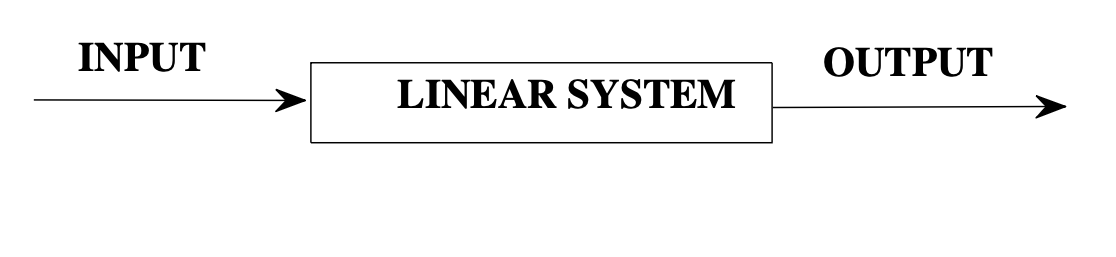
\includegraphics[width=0.8\textwidth]{Chapter 1/fig1-9.png}
	\caption{Schematic representation of a linear system.}
	\label{fig:1.9}
\end{figure}

Given a time series, we may want to predict future values based on the current and past values, for example in sales forecasting. Here we are doing `prediction' and `forecasting'.

\textit{(iv) Control}

Time series are sometimes collected to improve control over some physical or economic system. For example, if a time series is used to keep track of the quality of manufacturing, we would want it to always be at the `high' level. Control problems are related to predictions, as we can use predictions for error correction.

This topic is only briefly touched on in Section 14.3.



% ----------1.4----------
\subsection{Approaches to Time Series Analysis}
This book describes various approaches to time series: 
\begin{itemize}
	\item Chapter 2: Simple descriptive techniques (plotting, trend and seasonality, etc.)
	\item Chapter 3: Probability models for time series
	\item Chapter 4: Fitting models to time series
	\item Chapter 5: Forecasting procedures
	\item Chapter 6: Spectral density function
	\item Chapter 7: Using spectral analysis to estimate the spectral density function
	\item Chapter 8: Analysis of bivariate time series
	\item Chapter 9: Using linear systems 
	\item Chapter 10: State-space models + Kalman filter
	\item Chapter 11: Nonlinear time series analysis
	\item Chapter 12: Volatility time series model analysis
	\item Chapter 13: Multivariate time series model analysis
	\item Chapter 14: More advanced stuff!
\end{itemize}



% ----------1.5----------
\subsection{Review of Books on Time Series}
This subsections simply concerns other books on time series that may be helpful. The complete list is here:


